% !TEX root = Dokumentation.tex
\subsection{Team}

\begin{minipage}{0.49\textwidth}
\begin{flushleft} \large
\emph{Maschinenbau}\\
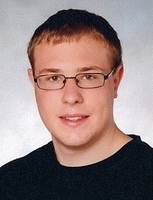
\includegraphics[width=0.3\textwidth]{./04_Projektmanagement/fig/stefanhaefliger.jpg}\\
Stefan Häfliger\\
Beladen und Entladen\\
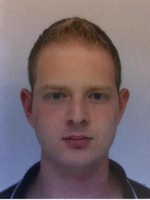
\includegraphics[width=0.3\textwidth]{./04_Projektmanagement/fig/joelmeloni.jpg}\\
Joël Meloni\\
Chassis und Lenkung\\
\emph{Elektrotechnik}\\
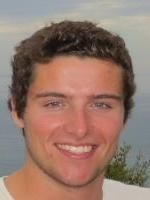
\includegraphics[width=0.3\textwidth]{./04_Projektmanagement/fig/silvanritz.jpg}\\
Silvan Ritz\\
Servos, Sensoren und Freescale-Board\\
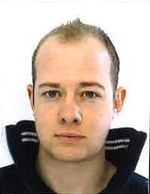
\includegraphics[width=0.3\textwidth]{./04_Projektmanagement/fig/larswalther.jpg}\\
Lars Walther\\
Energieversorgung und Antrieb\\
\end{flushleft}
\end{minipage}
\hfill
\begin{minipage}{0.49\textwidth}
\begin{flushright} \large
\emph{Informatik}\\
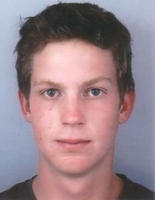
\includegraphics[width=0.3\textwidth]{./04_Projektmanagement/fig/patriziobrantschen.jpg}\\
Patrizio Brantschen\\
Objekterkennung und Rechtsvortritt\\
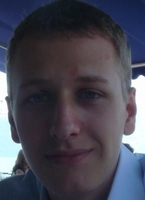
\includegraphics[width=0.3\textwidth]{./04_Projektmanagement/fig/adrianwuersch.jpg}\\
Adrian Würsch\\
Schnittstellen und Dokumentation\\
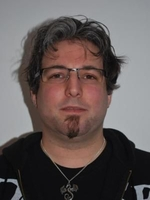
\includegraphics[width=0.3\textwidth]{./04_Projektmanagement/fig/tobiaskreienbuehl.jpg}\\
Tobias Kreienbühl\\
Fahrbahnerkennung und Mini-Computer\\
\end{flushright}
\end{minipage}









